% CausalVis paper, CVPR 2027 submission draft.
% Compile in Overleaf: open the official CVPR author kit, then replace its main.tex with this
% file and add refs.bib and the figures/ folder. Without cvpr.sty the fallback below still
% compiles, so the draft can be read before the kit is added.
\documentclass[10pt,twocolumn,letterpaper]{article}

\IfFileExists{cvpr.sty}{%
  \usepackage[review]{cvpr}%
}{%
  % CVPR-like page geometry, so the page count here matches the real template
  \usepackage[letterpaper,top=1in,bottom=1.125in,left=0.8125in,right=0.8125in,
              columnsep=0.3125in]{geometry}%
  \usepackage{times}%
  \usepackage[numbers,sort&compress]{natbib}%
  \newcommand{\cvprPaperID}{*****}%
}
\usepackage{graphicx}
\usepackage{amsmath,amssymb}
\usepackage{booktabs}
\usepackage{multirow}
\usepackage{xcolor}
\usepackage[hidelinks]{hyperref}
\def\UrlBreaks{\do\/\do-}
\usepackage[capitalize]{cleveref}
\usepackage{pdfpages}
\raggedbottom  % do not stretch a short column to the full height
\providecommand{\etal}{et al.}

\newcommand{\sys}{CausalVis}
\newcommand{\figfile}[2]{\IfFileExists{figures/#1}{\includegraphics{figures/#1}}{\fbox{\parbox[c][#2][c]{0.95\linewidth}{\centering\small figure file \texttt{#1} (see FIGURES.md)}}}}

% Set \anontrue for a double-blind submission (CVPR, NeurIPS). With the official
% cvpr.sty the [review] option already hides the author block, so this only matters
% for the fallback layout and for the arXiv version.
\newif\ifanon
\anonfalse

\title{Better Physics, Same Score: What an Auditable Counterfactual Engine\\Reveals About CLEVRER}
\ifanon
  \author{Anonymous submission}
\else
  \author{Syed Hamza Mukhtar Bukhari\\
  Faculty of Computer Science and Engineering\\
  Ghulam Ishaq Khan Institute of Engineering Sciences and Technology, Topi, Pakistan\\
  {\tt\small u2023682@giki.edu.pk}}
\fi
\date{}

\begin{document}
\maketitle

% =====================================================================================
\begin{abstract}
Counterfactual questions about video, such as ``what would happen if this object were removed?'', are a standard test of physical and causal reasoning, and CLEVRER is the most widely used benchmark for them.
However, a score on this benchmark shows neither which part of a system earned it nor whether a correct answer rests on a real event.
In this work, we present \sys{}, a counterfactual engine that answers by intervention.
It removes the object, keeps every other object on its recorded path until the change can reach it, hands the reached objects to a simulator, and returns the event that decided each answer.
The engine is never trained on questions or answers, and any simulator can be plugged into it.
We use it to audit CLEVRER on 1,398 held-out videos.
Across 13 simulators, a 2.2$\times$ range in rollout error moves the counterfactual score by only 2.2 points, and on predictive questions the most accurate simulator scores lowest.
Two choices that involve no physics matter more: when objects are handed to the simulator (1.2 points) and whether the simulation continues past the end of the video (4.6 points).
Of the correct answers that can be checked against the annotation, 98.2\% rest on a real recorded event.
We also find that CLEVRER's ``responsible'' labels contradict its own counterfactual answers in 35\% of cases, while a counterfactual test agrees better with human judgments.
Code, checkpoints and the per-answer records of every reported run are at {\small \url{https://github.com/bukhari-hamzamukhtar/CausalVis}}.
Our study suggests that counterfactual video benchmarks should report the evidence behind each answer alongside its accuracy.
\end{abstract}

% =====================================================================================
\section{Introduction}
\label{sec:intro}

Reasoning about what would have happened is central to physical understanding~\cite{battaglia2013simulation,gerstenberg2021csm}.
CLEVRER~\cite{yi2020clevrer} made it a benchmark: 20,000 synthetic videos of colliding objects, with questions such as ``What will happen if the cube is removed?''.
Methods for these counterfactual questions range from neuro-symbolic programs with learned dynamics~\cite{yi2020clevrer,chen2021dcl} to differentiable physics~\cite{ding2021vrdp} and end-to-end transformers~\cite{ding2021aloe}, and the best system answers 96.1\% of options correctly~\cite{ishay2024crcg}.

However, an accuracy number does not tell us which part of a system earned it, or whether a correct answer was reached for the right reason.
Recent audits show why this matters.
Frontier vision-language models often answer CLEVRER questions correctly without grounding in perception or physics~\cite{bagdonaviciute2025physics}, and 35\% of the correct answers of mid-tier models rest on physically invalid traces~\cite{bourigault2026words}.
Audits of other video benchmarks found that single frames or shortcuts explain much of the score~\cite{buch2022revisiting,krojer2025mvp,radsch2026verified}.
For CLEVRER, Ding \etal~\cite{ding2021aloe} observed that about half of the counterfactual questions remove an object that never collides.
What the counterfactual score measures has not been tested directly.

In this work, we build \sys{}, an engine that answers counterfactual questions with the three steps of a counterfactual~\cite{pearl2009causality}: abduction, action and prediction.
The recording plays the role of abduction: every object follows its recorded path until the intervention can reach it.
The action is the edit, for example the removal of an object.
For prediction, each reached object is handed to a simulator a few frames before it would lose a recorded contact, and the world is simulated past the end of the video.
The engine is never trained on questions or answers.
The simulator is a module: we use a small learned world model (43k parameters, trained on object motion only), textbook laws fitted to training videos, and straight-line motion.
Every answer comes with the event that decided it: the two objects, the frame, and whether the event was recorded or simulated.
Simulating only the objects an intervention affects was introduced by CRCG~\cite{ishay2024crcg}; we build on that idea and study when to hand objects over and how far to simulate.

We use the engine to audit CLEVRER's counterfactual questions on 1,398 held-out videos, with every setting chosen on a separate validation split and each test run made once.
With the learned world model, \sys{} answers 90.4\% of options and 72.3\% of questions; with fitted laws it answers 91.4\% and 75.0\%.
Across 13 simulators, the rollout error changes by a factor of 2.2 and the score by 2.2 points, because four very different simulators give the same answer on 91.4\% of options; on predictive questions the ranking of simulators reverses.
The score depends far more on the hand-off timing and on events after the last frame: 34.6\% of the questions whose removed object never collides need a collision that happens after the video ends.
For the correct answers whose deciding event can be checked, 98.2\% rest on a real recorded event, and on ComPhy, where the future is annotated, 97.7\% of correct predictive answers rest on a real future event.
Finally, CLEVRER's explanatory labels often call an object ``responsible'' for a collision that, according to CLEVRER's own counterfactual answers, still happens without that object (35.3\% of cases).
A counterfactual test matches human causal judgments~\cite{mao2022clevrerhumans} better than CLEVRER's rule.

In short, we make the following contributions:
\begin{itemize}
\item \textbf{An auditable counterfactual engine.} \sys{} answers by explicit intervention and simulation, takes any simulator, needs no question-answer training, and returns the deciding event of every answer (\cref{sec:method}).
\item \textbf{A controlled audit of CLEVRER.} With 13 simulators, one-change ablations and paired tests, we show that physical accuracy explains little of the counterfactual score and identify what it does depend on (\cref{sec:audit}).
\item \textbf{A measurement of answer validity.} We check the evidence behind each answer against the annotation on CLEVRER, against the annotated future on ComPhy~\cite{chen2022comphy} and against the true counterfactual trajectories on CoPhy~\cite{baradel2020cophy} (\cref{sec:evidence}).
\item \textbf{A finding on causal labels.} CLEVRER's ``responsible'' follows the chain of events; a counterfactual test disagrees with it and agrees better with people (\cref{sec:responsible}).
\end{itemize}
All training and evaluation ran on a single laptop CPU. Code, the split and the per-option records will be released.

% =====================================================================================
\section{Related work}
\label{sec:related}

\paragraph{Counterfactual reasoning about video.}
CLEVRER~\cite{yi2020clevrer} pairs synthetic collision videos with descriptive, explanatory, predictive and counterfactual questions.
NS-DR~\cite{yi2020clevrer} and DCL~\cite{chen2021dcl} execute question programs on object tracks and roll a learned dynamics model forward.
VRDP~\cite{ding2021vrdp} fits a differentiable rigid-body simulator to each video, ALOE~\cite{ding2021aloe} answers with a transformer over object embeddings, and SlotFormer~\cite{wu2023slotformer} rolls object slots forward for predictive questions.
CRCG~\cite{ishay2024crcg} keeps unaffected objects on their perceived states and simulates only the objects an intervention reaches, which raised VRDP from 94.8\% to 96.1\% per option.
Rovai~\cite{rovai2026eventgraph} replays the annotated event log without the removed object and notes that new collisions caused by a removal need a simulator.
Concurrently, PhysMind~\cite{yang2026physmind} builds one reusable executable world per video from segmentation, meshes and 6D pose, fits analytic dynamics to it and then inspects, continues or edits that world to answer a question, without training; it reports a 38.2 point gain over chain-of-thought prompting of the same vision-language model on CLEVRER.
We share the one-world-per-video design and the separation of perception from answering, and differ in what we do with it: our simulator is interchangeable, and we use the engine to measure how much of the benchmark score the physics explains.
Beyond CLEVRER, ComPhy~\cite{chen2022comphy} adds hidden mass and charge, CoPhy~\cite{baradel2020cophy,janny2022filtered} asks for counterfactual trajectories under hidden confounders, and CLEVRER-Humans~\cite{mao2022clevrerhumans} collects human causal judgments.
Other benchmarks test causal consistency~\cite{ates2022craft,foss2025causalvqa,begiristain2026cronos} or physical prediction~\cite{bear2021physion,tung2023physionpp,bordes2025intphys2}; Melnik \etal~\cite{melnik2023benchmarks} survey them.

\paragraph{Learned physical simulators.}
Graph-based simulators learn pairwise messages or forces~\cite{battaglia2016interaction,li2019propnet,sanchez2020gns}.
Energy-based networks conserve energy by construction~\cite{greydanus2019hnn,cranmer2020lnn,sanchez2019hgn,wang2026moshwm}, which makes friction and contact hard to represent~\cite{sosanya2022dissipative,gruver2022deconstructing}; built-in momentum conservation reduces long-horizon error~\cite{sharma2026dynamical} and contact-aware models handle rigid bodies~\cite{allen2023fignet}.
Inverse graphics recovers physical state by matching a renderer to images~\cite{wu2015galileo,wu2017deanimation}, and recent work reads rigid-body state and material out of video with a vision-language model~\cite{kao2026dynamics}.
Our learned simulator follows the energy-based line and adds friction by operator splitting~\cite{hairer2006geometric}.

\paragraph{Auditing benchmarks and answers.}
Buch \etal~\cite{buch2022revisiting} showed that a model which sees a single frame does well on many video-language tasks; minimal video pairs~\cite{krojer2025mvp} remove such shortcuts, and Physics-IQ Verified~\cite{radsch2026verified} audits a benchmark for video generators~\cite{motamed2026physicsiq}.
Video generators fail to learn physical laws outside their training data~\cite{kang2025howfar}, while self-supervised video models show some intuitive physics~\cite{garrido2025intuitive}.
Vision-language models answer physics questions without grounding~\cite{chow2025physbench,bagdonaviciute2025physics,bourigault2026words}.
Grounding language models in a simulator improves physical reasoning~\cite{liu2023mindseye,cherian2026llmphy,balazadeh2025pcb}.
We audit both the benchmark and our own answers.

\paragraph{Actual causation.}
The but-for test calls $C$ a cause of $E$ if $E$ would not have happened without $C$~\cite{lewis1973causation}; structural accounts refine it~\cite{halpern2005causes,halpern2016actual}.
People judge causation in collision scenes by simulating the counterfactual world~\cite{gerstenberg2021csm}, and learned models can support counterfactual inference when the abduction step is tractable~\cite{pawlowski2020deepscm,schoelkopf2021toward}.
CLEVRER instead labels causes with a rule over the chain of events, and CLEVRER-Humans~\cite{mao2022clevrerhumans} found that these labels differ from human judgments.

% =====================================================================================
\section{\sys{}}
\label{sec:method}

\begin{figure*}[t]
\centering
\figfile{fig1_teaser.pdf}{2.0in}
\caption{A counterfactual question answered with evidence. The top row shows the recorded video; the bottom row shows the world that \sys{} builds without the cube. Without the cube the red sphere keeps its path, misses the cylinder at frame 54 and strikes the gray sphere at frame 66. Each answer comes with the event that decided it (TEST-A video 10880, question 14).}
\label{fig:teaser}
\end{figure*}

\cref{fig:teaser} shows the engine on one question, and \cref{fig:method} shows its parts.

\paragraph{Tracks from video.}
We use the object detections released with NS-DR~\cite{yi2020clevrer}: Mask R-CNN~\cite{he2017maskrcnn} masks with predicted colour, material and shape.
Detections are linked into tracks by identity.
Each mask centre is lifted to the table plane with a camera that we recovered by fitting rendered silhouettes of the three CLEVRER shapes to the masks (median silhouette IoU 0.93).
The tracker finds 99.4\% to 99.8\% of the annotated objects with 99.4\% to 99.7\% precision on every split, and no annotation is read at test time (Supp.~B).

\paragraph{Interventions and reach.}
Let $x_i(t)$ be the recorded position of object $i$ at frame $t$, and let $\mathcal{C}$ be the set of objects an intervention changes (for a removal, the removed object).
An object is \emph{reached} at the first frame at which one of two things happens.
Either it would lose a recorded contact with an object in $\mathcal{C}$ or with an object already being simulated (\emph{lost contact}), or a simulated object touches it (\emph{new contact}).
Until then it follows $x_i(t)$ exactly.
This is the rule of CRCG~\cite{ishay2024crcg}, applied here to tracks.
Following the recording is the abduction step: it carries everything about the scene that the simulator does not model.

\paragraph{Hand-off.}
An object reached by a lost contact is handed to the simulator $L$ frames before that contact, with the position recorded at that frame and the mean velocity of the last three recorded frames; an object reached by a new contact is handed over at that frame.
We use $L=3$, chosen on validation (\cref{sec:audit}).
Objects that entered the view fewer than 15 frames earlier are partly outside the frame and appear at about 70\% of their speed.
For them we divide the velocity by a speed profile fitted on training tracks.
The counterfactual world runs $E$ frames past the end of the video ($E=30$ for the learned model, chosen on validation).

\paragraph{Simulators.}
We compare four simulators inside the same engine.
The \emph{learned world model} predicts a pair energy $V_\theta(x_i - x_j, a_i, a_j)$ from positions and attribute embeddings $a_i$.
The force on object $i$ is
\begin{equation}
F_i = -\sum_{j \neq i} \nabla_{x_i} V_\theta(x_i - x_j, a_i, a_j),
\end{equation}
computed by automatic differentiation.
Because $V_\theta$ depends on the difference of positions, $F_{ij} = -F_{ji}$ and momentum is conserved exactly.
Motion advances by leapfrog steps wrapped in exact friction half-steps $p_i \leftarrow p_i\, e^{-\gamma_i \Delta t/2}$ (Strang splitting~\cite{hairer2006geometric}), with a learned friction coefficient $\gamma_i$ per object.
Collisions receive an impulse along the contact normal~\cite{mirtich1995impulse}, which is estimated from voxelised object surfaces.
The model has 43,460 parameters and was trained on the tracks of 11,182 training videos with a 20-frame rollout loss; it never sees a question or an answer.
The \emph{textbook laws} use constant deceleration for sliding cubes and cylinders, exponential damping for rolling spheres and an impulse along the line of centres, with constants fitted on training tracks.
\emph{Straight lines} move each object at its hand-off velocity, with or without the fitted friction.
\emph{No physics} deletes the removed object and keeps every other object on its recording.

\paragraph{Events and evidence.}
Two objects collide at frame $t$ if their surfaces are closer than a calibrated margin (radii scaled by 1.2, plus 0.03).
They also collide if they are within 0.03 and one of them changes velocity by at least 0.002 within 6 frames.
An option such as ``the cylinder and the sphere collide'' is answered yes if the counterfactual world contains such an event, and the answer is flipped for questions asking what will \emph{not} happen.
For every option the engine stores the deciding event (the first collision of the asked pair, or its absence) and whether both objects still followed the recording at that frame.
This record is the evidence we audit in \cref{sec:evidence}.

\paragraph{Other question types.}
For descriptive, explanatory and predictive questions we run CLEVRER's question programs on the recorded events with the semantics of the NS-DR executor, and predictive questions simulate the scene past the end with no intervention.
Programs come from templates learned on training questions, which reproduce the dataset's counterfactual programs exactly on the validation split (Supp.~B).

\begin{figure*}[t]
\centering
\figfile{fig2_method.pdf}{1.3in}
\caption{\sys{}. Tracks come from detections and the parsed question sets the intervention. Objects follow the recorded video until the intervention can reach them, and are then handed to a simulator, which can be swapped. The supplement shows the same pipeline running on the example of \cref{fig:teaser}.}
\label{fig:method}
\end{figure*}

% =====================================================================================
\section{Experimental setup}
\label{sec:setup}

\paragraph{Splits.}
CLEVRER's test server closed on 16 January 2026 and our requests to the organisers went unanswered, so the answers of its test set are not available to us.
Before any experiment we fixed a split of the 15,000 videos that have answers.
TEST-A holds 500 CLEVRER validation videos (930 counterfactual questions, 3,332 options) and TEST-B holds 898 CLEVRER training videos that we trained nothing on (1,689 questions, 6,018 options).
One caveat belongs here rather than in a footnote: our perception reads NS-DR's detector, which its authors trained on CLEVRER training videos, so TEST-B is held out for our engine and its world model but not for that detector.
The two sets score within 0.3 points of each other throughout, which is what we would expect if this did not decide anything, and TEST-A carries no such caveat.
VAL-A holds another 500 validation videos (941 questions, 3,391 options) and is used for every choice of setting.
The world model and the laws were fitted on 11,182 other training videos.

\paragraph{Protocol.}
We wrote down the systems and settings to be tested before the test runs (Supp.~A).
For each simulator, the look-ahead $L \in \{1,3,6,12\}$, the collision detector and the extension $E \in \{0,10,20,30,45,60\}$ were chosen on VAL-A by the number of correct options, and each test run was made once.
We report accuracy per option and per question (a question is correct when all its options are).
Intervals are 95\% bootstrap intervals over videos with 2,000 resamples~\cite{efron1993bootstrap}, and paired comparisons use McNemar's test~\cite{mcnemar1947note} on the same options, reported as $z$ (so $|z|>1.96$ corresponds to $p<0.05$).

\paragraph{Physical accuracy.}
For every simulator we start from true states on 200 VAL-A videos and measure the mean position error after 40 frames, which we call the rollout error.
Besides the four simulators we evaluate nine checkpoints of the learned model from earlier training runs; six retrained seeds are evaluated on the benchmark only.

\paragraph{Compute.}
Every experiment ran on one laptop CPU (Intel i5-8350U, 4 cores, 7.9 GB of memory) without a GPU.
Training the world model took 8.1 hours, and answering a counterfactual question takes 2.2 seconds with the learned model and 1.4 seconds with the laws (one process, one thread).

% =====================================================================================
\section{Results}
\label{sec:results}

\begin{table}[tb]
\caption{Counterfactual questions on CLEVRER. Accuracy per option and per question. Published numbers are on the official test set. Ours are on 1,398 held-out videos (TEST-A and TEST-B pooled), and the last column gives the fresh TEST-B set alone, which our pre-registration names as primary. $\dagger$: trained object detector; $\ddagger$: attribute labels in training. $\ast$: concurrent, measured on its own fixed subset of 1,000 CLEVRER validation scenes rather than the test set, and training-free apart from off-the-shelf perception. The rows of \sys{} share the engine and differ only in the simulator.}
\label{tab:main}
\centering
\small
\setlength{\tabcolsep}{3pt}
\begin{tabular}{@{}lcccc@{}}
\toprule
Method & Sup. & Option & Question & TEST-B \\
\midrule
NS-DR~\cite{yi2020clevrer} & $\dagger\ddagger$ & 74.1 & 42.2 & \\
DCL~\cite{chen2021dcl} & $\dagger$ & 80.4 & 46.5 & \\
VRDP, no labels~\cite{ding2021vrdp} & none & 89.9 & 75.7 & \\
ALOE~\cite{ding2021aloe} & none & 91.4 & 75.6 & \\
VRDP~\cite{ding2021vrdp} & $\dagger\ddagger$ & 94.8 & 84.3 & \\
CRCG on VRDP~\cite{ishay2024crcg} & $\dagger\ddagger$ & 96.1 & 87.8 & \\
PhysMind~\cite{yang2026physmind}$^{\ast}$ & none & 88.1 & 70.6 & \\
\midrule
\sys{}, no physics & $\dagger\ddagger$ & 81.4 & 50.1 & 81.5 / 50.6 \\
\sys{}, straight lines & $\dagger\ddagger$ & 89.7 & 70.2 & 89.6 / 70.2 \\
\sys{}, straight + friction & $\dagger\ddagger$ & 90.2 & 71.9 & 90.2 / 72.2 \\
\sys{}, learned model & $\dagger\ddagger$ & 90.4 & 72.3 & 90.5 / 72.8 \\
\sys{}, textbook laws & $\dagger\ddagger$ & \textbf{91.4} & \textbf{75.0} & 91.3 / 74.8 \\
\bottomrule
\end{tabular}
\end{table}

\subsection{Main results}
\label{sec:main}

\cref{tab:main} compares \sys{} with published systems.
With the learned world model, \sys{} answers 90.4\% of options (95\% interval 89.7 to 91.1) and 72.3\% of questions (70.5 to 74.2).
The fitted laws answer 91.4\% and 75.0\%, 1.0 points above the learned model ($z=5.0$).
The two test sets agree: the learned model scores 90.2\% on TEST-A and 90.5\% on the fresh TEST-B, and the laws 91.7\% and 91.3\% ($z=3.1$ on TEST-B alone).
We report the pooled sets from here on, which narrows the intervals; the comparisons in this section hold on TEST-B alone (Supp.~J).
\sys{} stays 3.4 to 5.7 points per option below VRDP and CRCG, which use the same kind of perception.
The closest concurrent system, PhysMind~\cite{yang2026physmind}, also builds one editable world per video and reports 88.1 per option and 70.6 per question on its own 1,000-scene validation subset; it reaches that without any CLEVRER-trained perception, so the 2.3-point difference from our numbers is not a like-for-like gap in either direction.
Without any physics the engine already answers 81.4\% of options, above NS-DR and DCL; physics adds 9.0 points per option and 22.2 per question.
For the other direction, a general vision-language model given 16 frames of the video and the same options, Qwen2.5-VL-7B-Instruct~\cite{bai2025qwen25vl}, answers 54.4\% of options on TEST-A, which is what answering ``no'' to every event scores (54.1\%), and 2.9\% of questions (Supp.~C).

\subsection{What the counterfactual score measures}
\label{sec:audit}

\begin{figure*}[t]
\centering
\figfile{fig3_audit.pdf}{2.2in}
\caption{Physics quality against benchmark score. (a) On counterfactual questions a 2.2$\times$ spread in rollout error moves the score by 2.2 points, and most differences sit inside the 95\% intervals. (b) On predictive questions the order reverses: the most accurate simulator scores lowest. Hollow circles in (a) are nine further checkpoints of the learned model; across all 13 simulators Pearson $r = -0.59$, and the no-physics baseline (81.4) is below the axis. Error is measured on 200 VAL-A videos; scores on TEST-A and TEST-B.}
\label{fig:audit}
\end{figure*}

\paragraph{Better physics, same score.}
\cref{fig:audit}a plots the counterfactual score of 13 simulators against their rollout error.
The error ranges from 0.050 to 0.113, a factor of 2.2, while the score ranges from 89.2\% to 91.4\% (Pearson $r=-0.59$).
Straight lines have 1.8 times the rollout error of the learned model and score only 0.75 points lower.
Earlier checkpoints of the learned model range from 89.2\% to 90.9\%, a spread as large as most changes of simulator.
On predictive questions the relation reverses (\cref{fig:audit}b): straight lines answer 91.4\% of options and the laws, which have the lowest rollout error, answer 88.1\% ($z=-3.8$ against the learned model).
A physical simulator therefore does not guarantee a better score on either question type.
The claim is about accuracy above a low bar and not about physics as a whole: removing the simulation entirely costs 9.0 points per option, while making it 2.2 times more accurate buys at most 2.2.
The reason is visible in the answers themselves.
The four simulators give the same answer on 91.4\% of the 9,350 counterfactual options, although at least one asked object is simulated before the video ends on 47.8\% of them.
Every difference between simulators comes from the remaining 8.6\%, and there the laws are right on 67.5\% of options, the learned model on 55.7\% and straight lines on 47.0\%.
A yes-or-no question about a collision changes only when a trajectory error moves a pair across the contact distance, and this agreement suggests that most asked pairs are far from that boundary.

\begin{figure}[tb]
\centering
\figfile{fig4_changes.pdf}{3.2in}
\caption{Effect of each change on the full system. Points are paired differences in options correct on TEST-A and TEST-B with 95\% video-bootstrap intervals; filled markers exclude zero. The extension past the video end and the hand-off timing matter most; the learned parts matter little, and removing the learned pair energy helps.}
\label{fig:changes}
\end{figure}

\paragraph{What the score depends on.}
\cref{fig:changes} removes one part of the system at a time.
Stopping the simulation at the last frame costs 4.6 points per option and 14.3 per question.
Handing objects over 12 frames before the lost contact instead of 3 costs 1.2 and 3.2 points, and on VAL-A every simulator improves as the hand-off moves later (Supp.~D).
The contact impulse is worth 0.8 points and the path-change detector 0.3.
Removing the learned pair energy, so that objects interact only through contact impulses, improves the score by 0.4 points; the learned friction and the entry correction make no measurable difference.
The hand-off and the extension decide when simulation starts and how long the world lasts, and neither involves physics.

\paragraph{Collisions after the video ends.}
Following ALOE~\cite{ding2021aloe}, we split questions into those whose removed object never collides (48.2\%), those whose answers the recorded video already contains (22.9\%), and the rest (28.9\%), which need counterfactual reasoning.
On the last group no physics answers 5.3\% of questions, the learned model 56.6\% and the laws 63.2\% (Supp.~E).
In the first group nothing in the video changes, yet the answer key says that a pair collides on 474 options where the video shows no collision of that pair.
These options occur in 34.6\% of the questions of the group and can only be answered by simulating past the last frame, which explains why the extension matters.
The learned system gets 896 options wrong.
Of these, 40\% invent a collision during the video, 31\% miss one after the video ends and 16\% invent one after it; 10\% miss a visible collision and 4\% name an object the detector did not find.

\subsection{Are the answers right for the right reason?}
\label{sec:evidence}

\begin{figure*}[t]
\centering
\figfile{fig5_evidence.pdf}{2.1in}
\caption{The evidence behind each answer. (a) Most correct answers rest on an event that can be checked against CLEVRER's annotation, and 98.2\% of those checks pass; the rest are decided in simulation, where no ground truth exists. (b) The deciding collision is found a median of 4 frames before the annotated contact. (c) Reported events against true events: recorded CLEVRER videos, simulated CoPhy counterfactuals with 2 to 6 balls, and simulated ComPhy futures.}
\label{fig:evidence}
\end{figure*}

Each answer of \sys{} names its deciding event.
When both asked objects still follow the recording at that event, the event can be compared with CLEVRER's collision annotation, which the engine never reads.
\cref{fig:evidence}a shows the result for the learned system.
Of the 8,454 correct answers, 4,973 can be checked this way.
Of these, 4,881 (98.2\%) rest on a real event: an annotated collision of the same pair within 15 frames, or no collision of the pair in the whole video.
With a 6-frame tolerance the rate is 93.4\%, because our detector fires a median of 4 frames before the annotated contact (\cref{fig:evidence}b).
Another 40.5\% of correct answers are decided in the simulated part of the world, for which CLEVRER has no ground truth.
Bourigault~\cite{bourigault2026words} reports that 35\% of the correct answers of mid-tier vision-language models rest on invalid traces; for the checkable answers of \sys{} the rate is 1.8\%, although the two checks verify different things.

The evidence also explains errors.
Of the 305 wrong answers that can be checked, 188 come from a collision that the detector reports and the annotation does not contain, and 37 from an annotated collision that the detector misses.
In 72 more, the key places a collision after the end of the video and our extension does not reach it.
On the recorded videos, the event detector used for the other question types finds 95\% of the annotated collisions with 79\% precision (Supp.~F).

CoPhy~\cite{baradel2020cophy} provides the true counterfactual trajectory, so there the simulated events can be checked too.
We run the engine with the laws on BallsCF, infer the hidden masses and restitutions from the observed run, and compare the collisions in the predicted counterfactual run with the true ones (same pair, within one step).
With 2 balls, 85\% of the reported collisions are real and 65\% of the real ones are found; with 4 balls, 61\% and 49\%, and with 6 balls, 49\% and 41\% (\cref{fig:evidence}c).
Longer chains of collisions leave more room for a simulated event to drift, which is the same weakness that the counterfactual questions of CLEVRER expose.

ComPhy~\cite{chen2022comphy} annotates what happens after the end of each video, so there every predictive answer can be checked.
On 400 validation scenes, 1,378 of the 1,411 correct predictive answers (97.7\%) rest on a real future event: a collision of the same pair within 5 frames of the simulated one, or no collision of the pair at all.
The first simulated collision of an asked pair is real in 93.5\% of cases, and 76.9\% of the real ones are found.

\subsection{What ``responsible'' means}
\label{sec:responsible}

\begin{figure}[tb]
\centering
\figfile{fig6_responsible.pdf}{2.4in}
\caption{Two meanings of ``responsible''. (a) When CLEVRER's key marks an object responsible for a collision, its own counterfactual answers say the pair still collides without that object in 35.3\% of cases. (b) CLEVRER's chain rule (grey) matches CLEVRER's key; removing the cause and checking whether the collision still happens (blue) matches human judgments better.}
\label{fig:responsible}
\end{figure}

CLEVRER's explanatory questions ask which event is ``responsible'' for a collision.
The answer key follows a chain rule: an event is responsible if it precedes the collision in the chain of events of the objects involved~\cite{yi2020clevrer}.
The but-for test, the standard test in law and philosophy, reads it differently: an event is a cause when the target would not have happened but for that event~\cite{lewis1973causation,gerstenberg2021csm}.
We apply it by removing what the candidate cause adds, simulating that world with the engine, and checking whether the target collision still happens.
Both rules can be run on the same options.
On TEST-A and TEST-B, the chain rule on our recorded events answers 88.4\% of options and 79.7\% of questions, and the but-for test 77.7\% and 61.5\% ($z=-27.2$).

This gap is not only a simulation error.
To check this without any model, we paired explanatory and counterfactual options from the same video.
The explanatory option states that the presence (or entrance) of $Z$ is responsible for the collision of $X$ and $Y$, and the counterfactual option asks whether $X$ and $Y$ collide without $Z$.
Over VAL-A, TEST-A and TEST-B, the key calls $Z$ responsible in 320 such pairs.
In 113 of them (35.3\%, \cref{fig:responsible}a), CLEVRER's own counterfactual answer says that $X$ and $Y$ still collide without $Z$.
Where the key calls $Z$ not responsible, the two answers disagree in 1 of 1,366 pairs.
The counterfactual answer does not give the time of the collision, so a later collision of the same pair could explain some of these cases.
It explains few of them: in all 113 cases the pair collides only once in the recorded video, and in the engine's world without $Z$ the pair collides within 10 frames of that recorded collision in 56 cases.

Human judgments separate the two readings (\cref{fig:responsible}b).
CLEVRER-Humans~\cite{mao2022clevrerhumans} asks people which events cause which.
On it, the but-for test with \sys{} answers 64.4\% of options and the chain rule on the same events 60.9\%.
The best published model answers 54.0\%, and the human performance reported with the dataset is 84.5\%.
CLEVRER's explanatory score therefore rewards a rule that agrees less with people than the but-for test does.

\subsection{Other question types and benchmarks}
\label{sec:other}

\begin{table}[tb]
\caption{Other CLEVRER question types, per option and per question. Published numbers are on the official test set; ours on TEST-A and TEST-B.}
\label{tab:qtypes}
\centering
\small
\setlength{\tabcolsep}{3.5pt}
\begin{tabular}{@{}lccccc@{}}
\toprule
& Descr. & \multicolumn{2}{c}{Explanatory} & \multicolumn{2}{c}{Predictive} \\
Method & & Opt. & Ques. & Opt. & Ques. \\
\midrule
NS-DR~\cite{yi2020clevrer} & 88.1 & 87.6 & 79.6 & 82.9 & 68.7 \\
DCL~\cite{chen2021dcl} & 90.7 & 89.6 & 82.8 & 90.5 & 82.0 \\
ALOE~\cite{ding2021aloe} & 94.0 & 98.5 & 96.0 & 93.5 & 87.5 \\
VRDP~\cite{ding2021vrdp} & 93.4 & 96.3 & 91.9 & 95.7 & 91.4 \\
\midrule
\sys{} & 90.9 & 88.4 & 79.7 & 90.5 & 82.6 \\
\bottomrule
\end{tabular}
\end{table}

\cref{tab:qtypes} reports the other CLEVRER question types.
\sys{} is on par with DCL and below ALOE and VRDP.
Its predictive score uses the learned model, which was best on VAL-A; on the test sets straight lines scored 0.9 points higher.

On ComPhy~\cite{chen2022comphy}, where masses and charges are hidden, we infer them from the target video and its four reference videos and simulate with fitted laws.
With tracks taken from the annotation, the engine answers 79.5\% of counterfactual and 86.9\% of predictive options on the validation set, against 68.3\% and 75.3\% for CPL and 80.0\% and 88.0\% for people on the test set (Supp.~H).
On CoPhy BallsCF with 2 to 6 balls, its counterfactual position error is 0.89 to 2.60, between 12\% and 45\% of the error of copying the observed trajectory (Supp.~I).
Both use oracle tracks and show that the engine transfers; they are not comparable with methods that work from pixels.

% =====================================================================================
\section{Limitations}
\label{sec:limitations}

Our work has several limitations.
First, all scenes are synthetic, with three shapes, one object size and almost no occlusion; we did not test the engine on real video.
Second, our perception uses NS-DR's detector, which was trained with CLEVRER's masks and attributes, so the fair comparison group in \cref{tab:main} is VRDP and CRCG.
Third, the answers decided in simulation (40.5\% of the correct ones) can be inspected but not verified on CLEVRER.
Fourth, the simulators are planar and model neither toppling nor 3D rotation, and CLEVRER's test server had closed, so our test sets are held-out validation and training videos and the comparison with published numbers is approximate.
Finally, all training ran on one CPU, which limited how many times we could repeat it: the seven checkpoints of our recipe span 90.0 to 90.5 options correct (Supp.~C).
That spread is as large as several of the effects we report, which is itself part of our finding.

% =====================================================================================
\section{Conclusion}
\label{sec:conclusion}

We presented \sys{}, a counterfactual engine that answers by intervention and simulation and returns the event behind each answer.
Used as an instrument, it shows that CLEVRER's counterfactual score depends little on physical accuracy and much on when simulation starts and how long it runs, and that CLEVRER's causal labels follow a rule that people do not use.
For the answers we could check, the evidence was real in 98.2\% of cases.
We suggest that benchmarks for counterfactual reasoning report, next to accuracy, the share of answers that are decided by physics and the share whose evidence is valid.

\ifanon\else
% =====================================================================================
\section*{Acknowledgements}
I thank Dr. Khurram Khan Jadoon, Faculty of Computer Science and Engineering, Ghulam Ishaq Khan Institute of Engineering Sciences and Technology, who supervised the research internship from which this work grew.
His regular review of the design decisions, the results and the failure analyses set the direction the project took, and the standard he held for what a measurement has to show before it is believed is the habit this paper is built on.
I am grateful for his reading of a draft.

\paragraph{Use of AI assistance.}
An AI coding assistant was used for implementation support and for language editing of this manuscript: writing and refactoring code to a specification, drafting documentation, organising bibliographic records, and polishing prose.
The research question, the experimental design, the pre-registration, the choice of what to measure and the reading of every result are the author's own, and every number reported here was produced by code in the public repository and checked against the records deposited with it.
No text, citation or result was accepted without verification: each reference was checked against arXiv, Crossref or OpenAlex, and each claim traced to the run that produced it.
\fi

{\small
\IfFileExists{ieeenat_fullname.bst}{\bibliographystyle{ieeenat_fullname}}{\bibliographystyle{plainnat}}
\bibliography{refs}
}

\IfFileExists{supp.pdf}{\clearpage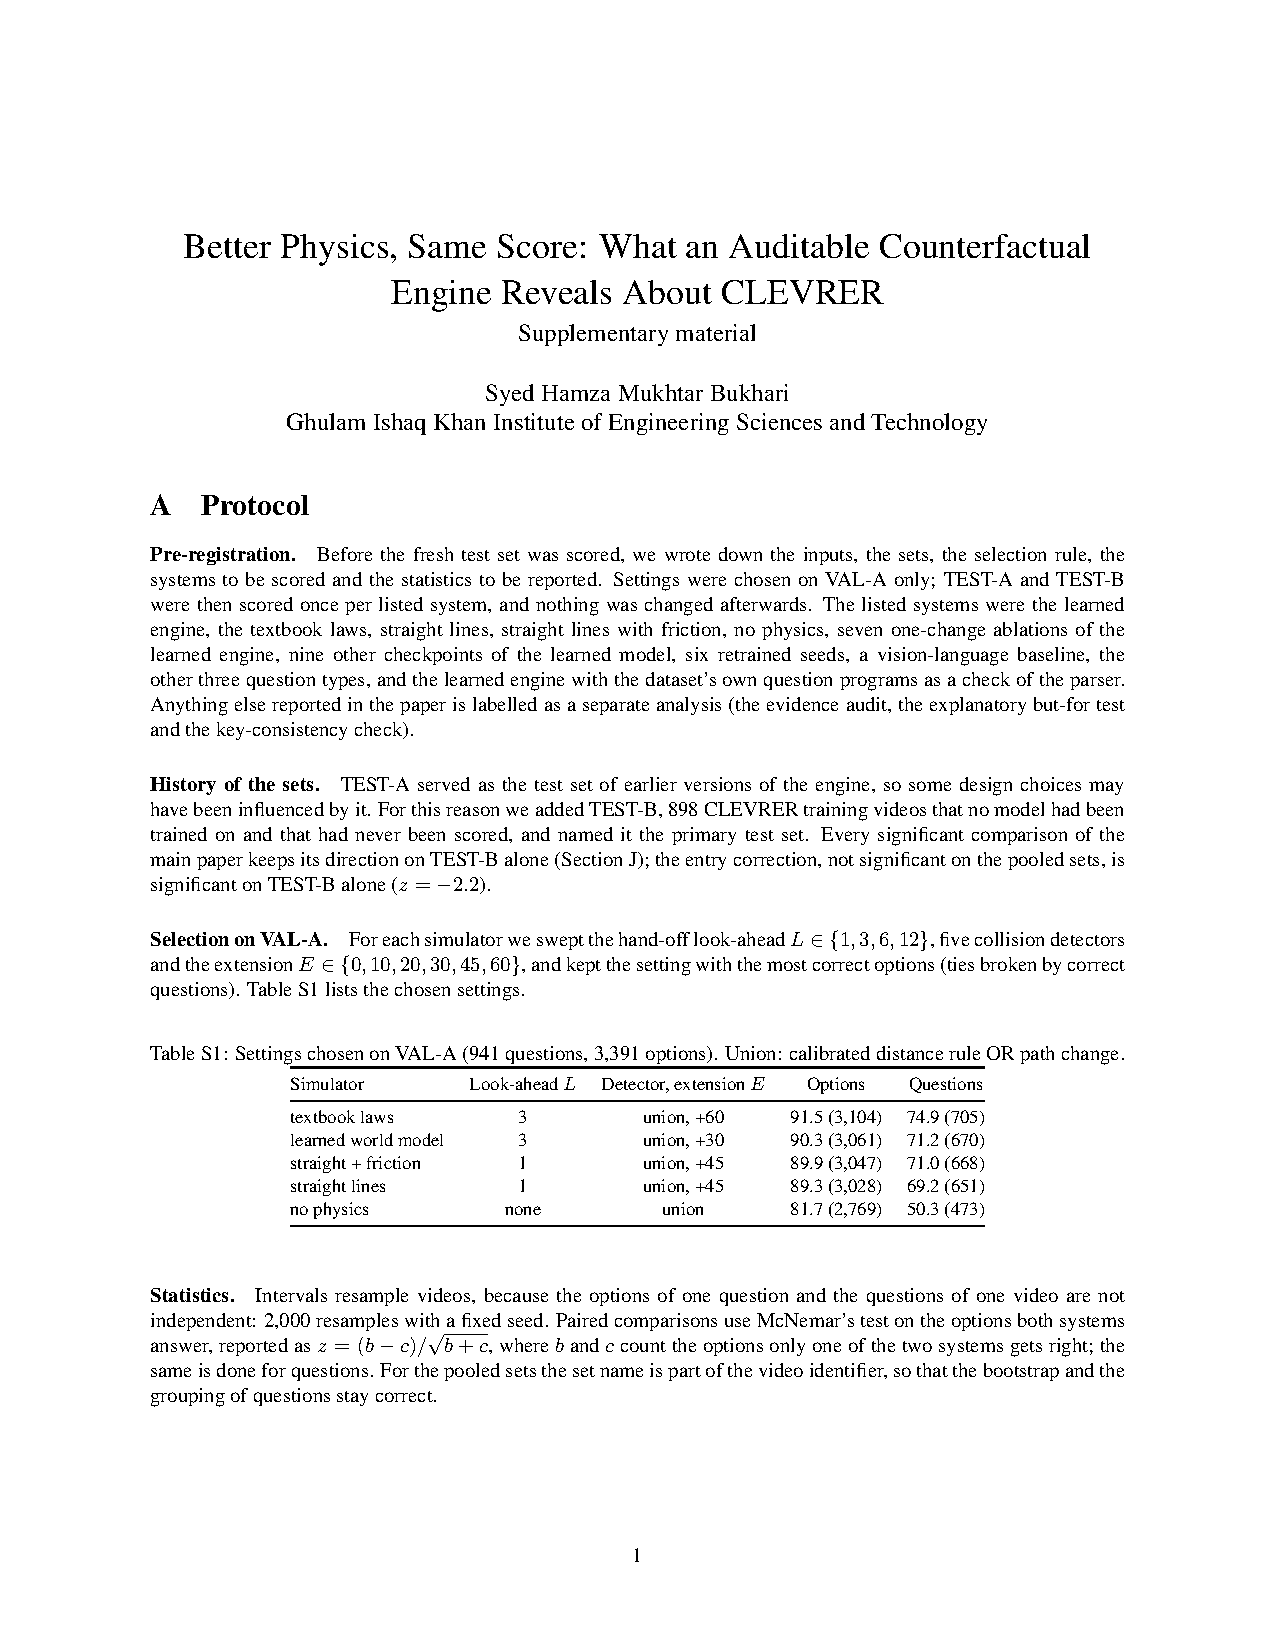
\includepdf[pages=-]{supp.pdf}}{}

\end{document}
